\documentclass[10pt]{article}
\usepackage{tmlr}
% Camera-ready only:
%\usepackage[accepted]{tmlr}
% To de-anonymize for a preprint:
%\usepackage[preprint]{tmlr}

%%%%% NEW MATH DEFINITIONS %%%%%

\usepackage{amsmath,amsfonts,bm}

% Mark sections of captions for referring to divisions of figures
\newcommand{\figleft}{{\em (Left)}}
\newcommand{\figcenter}{{\em (Center)}}
\newcommand{\figright}{{\em (Right)}}
\newcommand{\figtop}{{\em (Top)}}
\newcommand{\figbottom}{{\em (Bottom)}}
\newcommand{\captiona}{{\em (a)}}
\newcommand{\captionb}{{\em (b)}}
\newcommand{\captionc}{{\em (c)}}
\newcommand{\captiond}{{\em (d)}}

% Highlight a newly defined term
\newcommand{\newterm}[1]{{\bf #1}}


% Figure reference, lower-case.
\def\figref#1{figure~\ref{#1}}
% Figure reference, capital. For start of sentence
\def\Figref#1{Figure~\ref{#1}}
\def\twofigref#1#2{figures \ref{#1} and \ref{#2}}
\def\quadfigref#1#2#3#4{figures \ref{#1}, \ref{#2}, \ref{#3} and \ref{#4}}
% Section reference, lower-case.
\def\secref#1{section~\ref{#1}}
% Section reference, capital.
\def\Secref#1{Section~\ref{#1}}
% Reference to two sections.
\def\twosecrefs#1#2{sections \ref{#1} and \ref{#2}}
% Reference to three sections.
\def\secrefs#1#2#3{sections \ref{#1}, \ref{#2} and \ref{#3}}
% Reference to an equation, lower-case.
\def\eqref#1{equation~\ref{#1}}
% Reference to an equation, upper case
\def\Eqref#1{Equation~\ref{#1}}
% A raw reference to an equation---avoid using if possible
\def\plaineqref#1{\ref{#1}}
% Reference to a chapter, lower-case.
\def\chapref#1{chapter~\ref{#1}}
% Reference to an equation, upper case.
\def\Chapref#1{Chapter~\ref{#1}}
% Reference to a range of chapters
\def\rangechapref#1#2{chapters\ref{#1}--\ref{#2}}
% Reference to an algorithm, lower-case.
\def\algref#1{algorithm~\ref{#1}}
% Reference to an algorithm, upper case.
\def\Algref#1{Algorithm~\ref{#1}}
\def\twoalgref#1#2{algorithms \ref{#1} and \ref{#2}}
\def\Twoalgref#1#2{Algorithms \ref{#1} and \ref{#2}}
% Reference to a part, lower case
\def\partref#1{part~\ref{#1}}
% Reference to a part, upper case
\def\Partref#1{Part~\ref{#1}}
\def\twopartref#1#2{parts \ref{#1} and \ref{#2}}

\def\ceil#1{\lceil #1 \rceil}
\def\floor#1{\lfloor #1 \rfloor}
\def\1{\bm{1}}
\newcommand{\train}{\mathcal{D}}
\newcommand{\valid}{\mathcal{D_{\mathrm{valid}}}}
\newcommand{\test}{\mathcal{D_{\mathrm{test}}}}

\def\eps{{\epsilon}}


% Random variables
\def\reta{{\textnormal{$\eta$}}}
\def\ra{{\textnormal{a}}}
\def\rb{{\textnormal{b}}}
\def\rc{{\textnormal{c}}}
\def\rd{{\textnormal{d}}}
\def\re{{\textnormal{e}}}
\def\rf{{\textnormal{f}}}
\def\rg{{\textnormal{g}}}
\def\rh{{\textnormal{h}}}
\def\ri{{\textnormal{i}}}
\def\rj{{\textnormal{j}}}
\def\rk{{\textnormal{k}}}
\def\rl{{\textnormal{l}}}
% rm is already a command, just don't name any random variables m
\def\rn{{\textnormal{n}}}
\def\ro{{\textnormal{o}}}
\def\rp{{\textnormal{p}}}
\def\rq{{\textnormal{q}}}
\def\rr{{\textnormal{r}}}
\def\rs{{\textnormal{s}}}
\def\rt{{\textnormal{t}}}
\def\ru{{\textnormal{u}}}
\def\rv{{\textnormal{v}}}
\def\rw{{\textnormal{w}}}
\def\rx{{\textnormal{x}}}
\def\ry{{\textnormal{y}}}
\def\rz{{\textnormal{z}}}

% Random vectors
\def\rvepsilon{{\mathbf{\epsilon}}}
\def\rvtheta{{\mathbf{\theta}}}
\def\rva{{\mathbf{a}}}
\def\rvb{{\mathbf{b}}}
\def\rvc{{\mathbf{c}}}
\def\rvd{{\mathbf{d}}}
\def\rve{{\mathbf{e}}}
\def\rvf{{\mathbf{f}}}
\def\rvg{{\mathbf{g}}}
\def\rvh{{\mathbf{h}}}
\def\rvu{{\mathbf{i}}}
\def\rvj{{\mathbf{j}}}
\def\rvk{{\mathbf{k}}}
\def\rvl{{\mathbf{l}}}
\def\rvm{{\mathbf{m}}}
\def\rvn{{\mathbf{n}}}
\def\rvo{{\mathbf{o}}}
\def\rvp{{\mathbf{p}}}
\def\rvq{{\mathbf{q}}}
\def\rvr{{\mathbf{r}}}
\def\rvs{{\mathbf{s}}}
\def\rvt{{\mathbf{t}}}
\def\rvu{{\mathbf{u}}}
\def\rvv{{\mathbf{v}}}
\def\rvw{{\mathbf{w}}}
\def\rvx{{\mathbf{x}}}
\def\rvy{{\mathbf{y}}}
\def\rvz{{\mathbf{z}}}

% Elements of random vectors
\def\erva{{\textnormal{a}}}
\def\ervb{{\textnormal{b}}}
\def\ervc{{\textnormal{c}}}
\def\ervd{{\textnormal{d}}}
\def\erve{{\textnormal{e}}}
\def\ervf{{\textnormal{f}}}
\def\ervg{{\textnormal{g}}}
\def\ervh{{\textnormal{h}}}
\def\ervi{{\textnormal{i}}}
\def\ervj{{\textnormal{j}}}
\def\ervk{{\textnormal{k}}}
\def\ervl{{\textnormal{l}}}
\def\ervm{{\textnormal{m}}}
\def\ervn{{\textnormal{n}}}
\def\ervo{{\textnormal{o}}}
\def\ervp{{\textnormal{p}}}
\def\ervq{{\textnormal{q}}}
\def\ervr{{\textnormal{r}}}
\def\ervs{{\textnormal{s}}}
\def\ervt{{\textnormal{t}}}
\def\ervu{{\textnormal{u}}}
\def\ervv{{\textnormal{v}}}
\def\ervw{{\textnormal{w}}}
\def\ervx{{\textnormal{x}}}
\def\ervy{{\textnormal{y}}}
\def\ervz{{\textnormal{z}}}

% Random matrices
\def\rmA{{\mathbf{A}}}
\def\rmB{{\mathbf{B}}}
\def\rmC{{\mathbf{C}}}
\def\rmD{{\mathbf{D}}}
\def\rmE{{\mathbf{E}}}
\def\rmF{{\mathbf{F}}}
\def\rmG{{\mathbf{G}}}
\def\rmH{{\mathbf{H}}}
\def\rmI{{\mathbf{I}}}
\def\rmJ{{\mathbf{J}}}
\def\rmK{{\mathbf{K}}}
\def\rmL{{\mathbf{L}}}
\def\rmM{{\mathbf{M}}}
\def\rmN{{\mathbf{N}}}
\def\rmO{{\mathbf{O}}}
\def\rmP{{\mathbf{P}}}
\def\rmQ{{\mathbf{Q}}}
\def\rmR{{\mathbf{R}}}
\def\rmS{{\mathbf{S}}}
\def\rmT{{\mathbf{T}}}
\def\rmU{{\mathbf{U}}}
\def\rmV{{\mathbf{V}}}
\def\rmW{{\mathbf{W}}}
\def\rmX{{\mathbf{X}}}
\def\rmY{{\mathbf{Y}}}
\def\rmZ{{\mathbf{Z}}}

% Elements of random matrices
\def\ermA{{\textnormal{A}}}
\def\ermB{{\textnormal{B}}}
\def\ermC{{\textnormal{C}}}
\def\ermD{{\textnormal{D}}}
\def\ermE{{\textnormal{E}}}
\def\ermF{{\textnormal{F}}}
\def\ermG{{\textnormal{G}}}
\def\ermH{{\textnormal{H}}}
\def\ermI{{\textnormal{I}}}
\def\ermJ{{\textnormal{J}}}
\def\ermK{{\textnormal{K}}}
\def\ermL{{\textnormal{L}}}
\def\ermM{{\textnormal{M}}}
\def\ermN{{\textnormal{N}}}
\def\ermO{{\textnormal{O}}}
\def\ermP{{\textnormal{P}}}
\def\ermQ{{\textnormal{Q}}}
\def\ermR{{\textnormal{R}}}
\def\ermS{{\textnormal{S}}}
\def\ermT{{\textnormal{T}}}
\def\ermU{{\textnormal{U}}}
\def\ermV{{\textnormal{V}}}
\def\ermW{{\textnormal{W}}}
\def\ermX{{\textnormal{X}}}
\def\ermY{{\textnormal{Y}}}
\def\ermZ{{\textnormal{Z}}}

% Vectors
\def\vzero{{\bm{0}}}
\def\vone{{\bm{1}}}
\def\vmu{{\bm{\mu}}}
\def\vtheta{{\bm{\theta}}}
\def\va{{\bm{a}}}
\def\vb{{\bm{b}}}
\def\vc{{\bm{c}}}
\def\vd{{\bm{d}}}
\def\ve{{\bm{e}}}
\def\vf{{\bm{f}}}
\def\vg{{\bm{g}}}
\def\vh{{\bm{h}}}
\def\vi{{\bm{i}}}
\def\vj{{\bm{j}}}
\def\vk{{\bm{k}}}
\def\vl{{\bm{l}}}
\def\vm{{\bm{m}}}
\def\vn{{\bm{n}}}
\def\vo{{\bm{o}}}
\def\vp{{\bm{p}}}
\def\vq{{\bm{q}}}
\def\vr{{\bm{r}}}
\def\vs{{\bm{s}}}
\def\vt{{\bm{t}}}
\def\vu{{\bm{u}}}
\def\vv{{\bm{v}}}
\def\vw{{\bm{w}}}
\def\vx{{\bm{x}}}
\def\vy{{\bm{y}}}
\def\vz{{\bm{z}}}

% Elements of vectors
\def\evalpha{{\alpha}}
\def\evbeta{{\beta}}
\def\evepsilon{{\epsilon}}
\def\evlambda{{\lambda}}
\def\evomega{{\omega}}
\def\evmu{{\mu}}
\def\evpsi{{\psi}}
\def\evsigma{{\sigma}}
\def\evtheta{{\theta}}
\def\eva{{a}}
\def\evb{{b}}
\def\evc{{c}}
\def\evd{{d}}
\def\eve{{e}}
\def\evf{{f}}
\def\evg{{g}}
\def\evh{{h}}
\def\evi{{i}}
\def\evj{{j}}
\def\evk{{k}}
\def\evl{{l}}
\def\evm{{m}}
\def\evn{{n}}
\def\evo{{o}}
\def\evp{{p}}
\def\evq{{q}}
\def\evr{{r}}
\def\evs{{s}}
\def\evt{{t}}
\def\evu{{u}}
\def\evv{{v}}
\def\evw{{w}}
\def\evx{{x}}
\def\evy{{y}}
\def\evz{{z}}

% Matrix
\def\mA{{\bm{A}}}
\def\mB{{\bm{B}}}
\def\mC{{\bm{C}}}
\def\mD{{\bm{D}}}
\def\mE{{\bm{E}}}
\def\mF{{\bm{F}}}
\def\mG{{\bm{G}}}
\def\mH{{\bm{H}}}
\def\mI{{\bm{I}}}
\def\mJ{{\bm{J}}}
\def\mK{{\bm{K}}}
\def\mL{{\bm{L}}}
\def\mM{{\bm{M}}}
\def\mN{{\bm{N}}}
\def\mO{{\bm{O}}}
\def\mP{{\bm{P}}}
\def\mQ{{\bm{Q}}}
\def\mR{{\bm{R}}}
\def\mS{{\bm{S}}}
\def\mT{{\bm{T}}}
\def\mU{{\bm{U}}}
\def\mV{{\bm{V}}}
\def\mW{{\bm{W}}}
\def\mX{{\bm{X}}}
\def\mY{{\bm{Y}}}
\def\mZ{{\bm{Z}}}
\def\mBeta{{\bm{\beta}}}
\def\mPhi{{\bm{\Phi}}}
\def\mLambda{{\bm{\Lambda}}}
\def\mSigma{{\bm{\Sigma}}}

% Tensor
\DeclareMathAlphabet{\mathsfit}{\encodingdefault}{\sfdefault}{m}{sl}
\SetMathAlphabet{\mathsfit}{bold}{\encodingdefault}{\sfdefault}{bx}{n}
\newcommand{\tens}[1]{\bm{\mathsfit{#1}}}
\def\tA{{\tens{A}}}
\def\tB{{\tens{B}}}
\def\tC{{\tens{C}}}
\def\tD{{\tens{D}}}
\def\tE{{\tens{E}}}
\def\tF{{\tens{F}}}
\def\tG{{\tens{G}}}
\def\tH{{\tens{H}}}
\def\tI{{\tens{I}}}
\def\tJ{{\tens{J}}}
\def\tK{{\tens{K}}}
\def\tL{{\tens{L}}}
\def\tM{{\tens{M}}}
\def\tN{{\tens{N}}}
\def\tO{{\tens{O}}}
\def\tP{{\tens{P}}}
\def\tQ{{\tens{Q}}}
\def\tR{{\tens{R}}}
\def\tS{{\tens{S}}}
\def\tT{{\tens{T}}}
\def\tU{{\tens{U}}}
\def\tV{{\tens{V}}}
\def\tW{{\tens{W}}}
\def\tX{{\tens{X}}}
\def\tY{{\tens{Y}}}
\def\tZ{{\tens{Z}}}


% Graph
\def\gA{{\mathcal{A}}}
\def\gB{{\mathcal{B}}}
\def\gC{{\mathcal{C}}}
\def\gD{{\mathcal{D}}}
\def\gE{{\mathcal{E}}}
\def\gF{{\mathcal{F}}}
\def\gG{{\mathcal{G}}}
\def\gH{{\mathcal{H}}}
\def\gI{{\mathcal{I}}}
\def\gJ{{\mathcal{J}}}
\def\gK{{\mathcal{K}}}
\def\gL{{\mathcal{L}}}
\def\gM{{\mathcal{M}}}
\def\gN{{\mathcal{N}}}
\def\gO{{\mathcal{O}}}
\def\gP{{\mathcal{P}}}
\def\gQ{{\mathcal{Q}}}
\def\gR{{\mathcal{R}}}
\def\gS{{\mathcal{S}}}
\def\gT{{\mathcal{T}}}
\def\gU{{\mathcal{U}}}
\def\gV{{\mathcal{V}}}
\def\gW{{\mathcal{W}}}
\def\gX{{\mathcal{X}}}
\def\gY{{\mathcal{Y}}}
\def\gZ{{\mathcal{Z}}}

% Sets
\def\sA{{\mathbb{A}}}
\def\sB{{\mathbb{B}}}
\def\sC{{\mathbb{C}}}
\def\sD{{\mathbb{D}}}
% Don't use a set called E, because this would be the same as our symbol
% for expectation.
\def\sF{{\mathbb{F}}}
\def\sG{{\mathbb{G}}}
\def\sH{{\mathbb{H}}}
\def\sI{{\mathbb{I}}}
\def\sJ{{\mathbb{J}}}
\def\sK{{\mathbb{K}}}
\def\sL{{\mathbb{L}}}
\def\sM{{\mathbb{M}}}
\def\sN{{\mathbb{N}}}
\def\sO{{\mathbb{O}}}
\def\sP{{\mathbb{P}}}
\def\sQ{{\mathbb{Q}}}
\def\sR{{\mathbb{R}}}
\def\sS{{\mathbb{S}}}
\def\sT{{\mathbb{T}}}
\def\sU{{\mathbb{U}}}
\def\sV{{\mathbb{V}}}
\def\sW{{\mathbb{W}}}
\def\sX{{\mathbb{X}}}
\def\sY{{\mathbb{Y}}}
\def\sZ{{\mathbb{Z}}}

% Entries of a matrix
\def\emLambda{{\Lambda}}
\def\emA{{A}}
\def\emB{{B}}
\def\emC{{C}}
\def\emD{{D}}
\def\emE{{E}}
\def\emF{{F}}
\def\emG{{G}}
\def\emH{{H}}
\def\emI{{I}}
\def\emJ{{J}}
\def\emK{{K}}
\def\emL{{L}}
\def\emM{{M}}
\def\emN{{N}}
\def\emO{{O}}
\def\emP{{P}}
\def\emQ{{Q}}
\def\emR{{R}}
\def\emS{{S}}
\def\emT{{T}}
\def\emU{{U}}
\def\emV{{V}}
\def\emW{{W}}
\def\emX{{X}}
\def\emY{{Y}}
\def\emZ{{Z}}
\def\emSigma{{\Sigma}}

% entries of a tensor
% Same font as tensor, without \bm wrapper
\newcommand{\etens}[1]{\mathsfit{#1}}
\def\etLambda{{\etens{\Lambda}}}
\def\etA{{\etens{A}}}
\def\etB{{\etens{B}}}
\def\etC{{\etens{C}}}
\def\etD{{\etens{D}}}
\def\etE{{\etens{E}}}
\def\etF{{\etens{F}}}
\def\etG{{\etens{G}}}
\def\etH{{\etens{H}}}
\def\etI{{\etens{I}}}
\def\etJ{{\etens{J}}}
\def\etK{{\etens{K}}}
\def\etL{{\etens{L}}}
\def\etM{{\etens{M}}}
\def\etN{{\etens{N}}}
\def\etO{{\etens{O}}}
\def\etP{{\etens{P}}}
\def\etQ{{\etens{Q}}}
\def\etR{{\etens{R}}}
\def\etS{{\etens{S}}}
\def\etT{{\etens{T}}}
\def\etU{{\etens{U}}}
\def\etV{{\etens{V}}}
\def\etW{{\etens{W}}}
\def\etX{{\etens{X}}}
\def\etY{{\etens{Y}}}
\def\etZ{{\etens{Z}}}

% The true underlying data generating distribution
\newcommand{\pdata}{p_{\rm{data}}}
% The empirical distribution defined by the training set
\newcommand{\ptrain}{\hat{p}_{\rm{data}}}
\newcommand{\Ptrain}{\hat{P}_{\rm{data}}}
% The model distribution
\newcommand{\pmodel}{p_{\rm{model}}}
\newcommand{\Pmodel}{P_{\rm{model}}}
\newcommand{\ptildemodel}{\tilde{p}_{\rm{model}}}
% Stochastic autoencoder distributions
\newcommand{\pencode}{p_{\rm{encoder}}}
\newcommand{\pdecode}{p_{\rm{decoder}}}
\newcommand{\precons}{p_{\rm{reconstruct}}}

\newcommand{\laplace}{\mathrm{Laplace}} % Laplace distribution

\newcommand{\E}{\mathbb{E}}
\newcommand{\Ls}{\mathcal{L}}
\newcommand{\R}{\mathbb{R}}
\newcommand{\emp}{\tilde{p}}
\newcommand{\lr}{\alpha}
\newcommand{\reg}{\lambda}
\newcommand{\rect}{\mathrm{rectifier}}
\newcommand{\softmax}{\mathrm{softmax}}
\newcommand{\sigmoid}{\sigma}
\newcommand{\softplus}{\zeta}
\newcommand{\KL}{D_{\mathrm{KL}}}
\newcommand{\Var}{\mathrm{Var}}
\newcommand{\standarderror}{\mathrm{SE}}
\newcommand{\Cov}{\mathrm{Cov}}
% Wolfram Mathworld says $L^2$ is for function spaces and $\ell^2$ is for vectors
% But then they seem to use $L^2$ for vectors throughout the site, and so does
% wikipedia.
\newcommand{\normlzero}{L^0}
\newcommand{\normlone}{L^1}
\newcommand{\normltwo}{L^2}
\newcommand{\normlp}{L^p}
\newcommand{\normmax}{L^\infty}

\newcommand{\parents}{Pa} % See usage in notation.tex. Chosen to match Daphne's book.

\DeclareMathOperator*{\argmax}{arg\,max}
\DeclareMathOperator*{\argmin}{arg\,min}

\DeclareMathOperator{\sign}{sign}
\DeclareMathOperator{\Tr}{Tr}
\let\ab\allowbreak

\usepackage{graphicx}
\usepackage{hyperref}
\usepackage{url}

\title{Geometry Is a Label, Not a Knob:\\
Causally Separating Representational Dimensionality from OOD Generalization}

\author{\name Anonymous Authors \AND \addr Anonymous Affiliation}

\newcommand{\fix}{\marginpar{FIX}}
\newcommand{\new}{\marginpar{NEW}}

\def\month{MM}
\def\year{YYYY}
\def\openreview{\url{https://openreview.net/forum?id=XXXX}}

% Operator shorthands
\newcommand{\dfx}{D_{\mathrm{eff}}}
\newcommand{\psix}{\Psi_{\mathrm{eff}}}
\newcommand{\rfx}{R_{\mathrm{eff}}}
\newcommand{\recolor}{\textsc{recolor}}
\newcommand{\aniso}{\textsc{aniso}}
\newcommand{\isot}{\textsc{iso}}
\newcommand{\rot}{\textsc{rotate}}

% Auto-generated number macros + E3 paired table
% Auto-generated by code/paper3_tables.py -- DO NOT EDIT NUMBERS BY HAND
% NOTE: macro names must be LaTeX-safe (no digits in prefix);
% architecture keys are mapped below.
\newcommand{\eOneBaseR}{+0.97}
\newcommand{\eOneBaseSlope}{+0.1367}
\newcommand{\eOneGeoShare}{7.7\%}
\newcommand{\anisoDc}{-10.8}
\newcommand{\anisoDidp}{-12.7}
\newcommand{\anisoRelD}{44}
\newcommand{\isoDc}{-6.5}
\newcommand{\isoDd}{+5.8}
\newcommand{\rotMaxDc}{1.7}
\newcommand{\rotMaxDd}{0.21}
\newcommand{\recZeroDc}{+1.7}
\newcommand{\eThreeDc}{+1.7}
\newcommand{\eThreeP}{0.016}
\newcommand{\eThreePosN}{7}
\newcommand{\eThreeInferP}{0.016}
\newcommand{\rBBaseR}{+0.98}
\newcommand{\rBBaseSlope}{+0.1332}
\newcommand{\rBGeoShare}{3.3\%}
\newcommand{\rBAnisoDc}{-9.6}
\newcommand{\rCBaseR}{+0.98}
\newcommand{\rCBaseSlope}{+0.0869}
\newcommand{\rCGeoShare}{1.9\%}
\newcommand{\rCAnisoDc}{-11.9}
\newcommand{\sfnBaseR}{+0.89}
\newcommand{\sfnBaseSlope}{+0.0701}
\newcommand{\sfnGeoShare}{-8.3\%}
\newcommand{\sfnAnisoDc}{-13.1}
\newcommand{\rgBaseR}{+0.87}
\newcommand{\rgBaseSlope}{+0.1139}
\newcommand{\rgGeoShare}{6.0\%}
\newcommand{\rgAnisoDc}{-16.0}

% E3 paired table
\newcommand{\eThreePairedTable}{%
\begin{tabular}{@{}lccccc@{}}
\hline
Model & $c_{100}^{\mathrm{w}}$ & $c_{100}^{\mathrm{ctrl}}$ & $\Delta c_{100}$ & $\Delta$ id-probe & $\Delta$ head (inf.) \\
\hline
{\tt l0.125\_w0.0001\_s0} & 0.300 & 0.273 & +2.7 & +0.0 & -0.1 \\
{\tt l0.125\_w0.0002\_s2} & 0.286 & 0.230 & +5.6 & +0.0 & +0.0 \\
{\tt l0.125\_w2.5e-05\_s1} & 0.284 & 0.282 & +0.2 & +0.0 & -0.6 \\
{\tt l0.5\_w0.0001\_s1} & 0.180 & 0.160 & +2.0 & +0.0 & -0.3 \\
{\tt l0.5\_w0.0002\_s2} & 0.168 & 0.155 & +1.2 & +0.0 & -0.1 \\
{\tt l0.5\_w5e-05\_s2} & 0.179 & 0.148 & +3.1 & +0.0 & -0.2 \\
{\tt l1.0\_w2.5e-05\_s0} & 0.158 & 0.144 & +1.4 & +0.0 & -0.1 \\
{\tt l1.0\_w5e-05\_s0} & 0.119 & 0.120 & -0.0 & +0.0 & -0.1 \\
\hline
\end{tabular}}

% E1 endpoint table
\newcommand{\eOneEndpointTable}{%
\begin{tabular}{@{}lccc@{}}
\hline
Model & \aniso$(2)$ $\Delta c_{100}$ & \isot$(2)$ $\Delta c_{100}$ & \recolor$(0)$ $\Delta c_{100}$ \\
\hline
{\tt l0.125\_w0.0001\_s0} & -13.2 & -13.1 & +2.7 \\
{\tt l0.125\_w0.0002\_s2} & -10.7 & -10.8 & +5.6 \\
{\tt l0.125\_w2.5e-05\_s1} & -13.0 & -13.7 & +0.2 \\
{\tt l0.5\_w0.0001\_s1} & -10.8 & -5.9 & +2.0 \\
{\tt l0.5\_w0.0002\_s2} & -11.1 & -6.0 & +1.2 \\
{\tt l0.5\_w5e-05\_s2} & -9.9 & -6.6 & +3.1 \\
{\tt l1.0\_w2.5e-05\_s0} & -10.5 & -6.3 & +1.4 \\
{\tt l1.0\_w5e-05\_s0} & -8.6 & -4.8 & -0.0 \\
\hline
\end{tabular}}


\begin{document}

\maketitle

% TMLR requires a first-page disclosure that LLMs were used in preparing the
% submission.
\let\thefootnote\relax\footnotetext{\emph{Use of LLMs:} Large language models were used as writing and coding assistants in preparing this manuscript; all scientific content, analyses, and reported numbers were determined and verified by the authors. A detailed statement appears in the Use of AI tools section.}\let\thefootnote\arabic

\begin{abstract}
% One paragraph, TMLR style. Numbers from locked data (runs/v2/{e1,e3,e2_*,e5b,e6}),
% all generated by code/paper3_analysis.py + paper3_tables.py macros.
Representational geometry markers such as the effective dimension $\dfx$
correlate strongly with out-of-distribution (OOD) accuracy across trained
networks, and this observation has motivated proposals to \emph{intervene} on
geometry---expanding or contracting feature-space dimensionality---as a route
to better transfer. We ask whether the observed correlation licenses such
interventions, and answer negatively for the spectral marker family tested
here. Across 8 ResNet-18 training recipes
spanning a $2.4\times$ effective-dimension range, the observational correlation is
large and stable ($r = +0.97$), yet three causal tests uniformly fail to
support an interpretable causal reading. (i) \emph{Operator-separation}:
injecting spectral-shape-matched noise collapses CIFAR-100 transfer
monotonically with dose in 8/8 models (median $-5.4$, $-7.1$, $-10.8$\,pp at
$\alpha \in \{0.5, 1, 2\}$) while $\dfx$ stays essentially unchanged, and a
fully deterministic spectral rotation that preserves the covariance spectrum
changes nothing (max $|\Delta \text{acc}| =
1.7$\,pp); conversely, a zero-noise whitening operator that multiplies $\dfx$
by up to $8\times$ (median $2.3\times$) moves transfer by at most $+5.6$\,pp
(median $+1.7$, never negative). (ii)
\emph{Timing-separation}: the apparent benefit of formation-phase whitening
(median $+1.7$\,pp, 7/8 models) is decomposed by a preregistered
dose--response adjudication into a \emph{probe-conditioning} effect ---
fully reproduced by transforming the probe's own training space, absent when
the transformed representation is scored in the original space --- while
applying the identical operator \emph{at inference} to an unchanged head
consistently \emph{degrades} accuracy (7/8 models, $p=0.016$). (iii)
\emph{Architecture transfer}: the same dissociation replicates in every tested
family---ResNet-34/50, ShuffleNet-V2, and RegNetY-400M (16 further recipes)---with
the observational anchor at $r \ge 0.87$ everywhere, spectral-shape-matched
noise dropping transfer $9.6$--$16.0$\,pp in 16/16 models, and inference-time
geometric slopes between $-8\%$ and $6\%$ of the observational slope ---
sign-unstable across families, as expected for a null. The dissociation also covers a
second marker family (participation ratio, effective rank): anisotropic
noise pins $\dfx$ while \emph{raising} these markers by $\approx$30\%,
moving geometry toward the observationally ``better'' regime as transfer
collapses. Together these results are consistent with $\dfx$ acting as a
\emph{confounded label} of the training recipe rather than a manipulable
cause of generalization for the spectral marker family tested here: the
geometric causal path carries at most a small fraction of the observational
association (point estimate $7.7\%$; bootstrap 95\% CI $[0.9\%, 46\%]$;
cross-architecture shares are sign-unstable, $-8.3\%$ to $+6.0\%$), and a
direct noise channel
that geometry does not measure carries the observable harm. We discuss why
``intervene on the geometry'' methods therefore require re-derivation, and
which interventions (noise control) the dissociation does support.
\end{abstract}

\section{Introduction}
\label{sec:intro}

Geometric descriptors of trained representations---effective dimension,
radius, utility, spectral decay---correlate with out-of-distribution (OOD)
accuracy strongly enough to serve as training-free model-selection markers.
The correlation is large ($r \approx 0.9$ or higher in controlled settings),
replicates across architectures, and survives the statistical controls that
kill weaker candidates. The natural next step, drawn repeatedly in the
literature, is interventional: if low-$\dfx$ models generalize worse, one
should be able to \emph{change} $\dfx$---by whitening, expanding, or
regularizing the feature geometry---and move generalization accordingly.
Methods that reshape representation geometry for robustness implicitly make
this inferential step.

This paper asks whether the step is licensed, and answers negatively for the
strongest candidate marker. We take the effective dimension $\dfx$ from the
GLUE family of geometry markers, which has the largest and most stable
observational association with OOD accuracy in our controlled setting
($r = +0.97$ across a purpose-built recipe grid), and subject it to a
three-part causal battery that any geometry-to-generalization story should
pass: \emph{operator separation} (move $\dfx$ with different operator
families that hold everything else fixed), \emph{timing separation} (apply
the same operator during representation formation vs.\ at inference), and
\emph{architecture transfer} (replicate in families beyond the one the
observation was discovered in). All experiments were preregistered before
unblinding (Appendix~\ref{app:prereg}).

\paragraph{What we find.}
The three tests uniformly fail the causal reading.
\begin{enumerate}
\item \emph{Operator separation (\S\ref{sec:e1}).} A family of
spectral-shape-matched noise operators collapses transfer monotonically
with dose in 8/8 models (median $-5.4$, $-7.1$, $-10.8$\,pp at
$\alpha \in \{0.5, 1, 2\}$) while $\dfx$ stays essentially unchanged; a
deterministic spectral rotation preserves the covariance spectrum exactly
and moves nothing; and zero-noise whitening multiplies $\dfx$ by up to
$8\times$ while moving transfer by at most $+5.6$\,pp (median $+1.7$, never
negative).
The causal slope of transfer on $\dfx$ under geometry-only operators is
$+0.0105$ per unit---$7.7\%$ of the observational slope (bootstrap CI
$[0.9\%, 46\%]$; within-model permutation noise floor
$[-7\%, +7\%]$, with the point estimate at the floor's upper edge)---so even
the CI upper bound leaves over half of the observational association without
a causal geometric account, and the dominant causal channel that \emph{does}
move transfer (noise) acts with the wrong sign and carries no geometric
signature.
\item \emph{Timing separation (\S\ref{sec:e3}).} The identical whitening
operator applied during formation \emph{appears} to improve transfer
(median $+1.7$\,pp, 7/8 paired models, $p = 0.016$), but a preregistered
dose--response adjudication decomposes this into a probe-conditioning
effect: the full benefit is reproduced by transforming only the probe's
training space (no formation manipulation), is absent when the
whitened-formation representation is scored in the original space, and
vanishes under an MLP readout. Applied at inference to the unchanged
trained head, the same operator \emph{degrades} accuracy (7/8 negative,
$p = 0.016$). Neither phase behavior can be predicted from the static
value of $\dfx$, and neither constitutes acting on representation
geometry.
\item \emph{Architecture transfer (\S\ref{sec:e2}).} The observational
anchor replicates in ResNet-34 ($r = +0.98$), and so does the dissociation:
spectral-shape-matched noise drops transfer $9.6$\,pp (4/4 models, $\dfx$
shifts $\le 12\%$); zero-noise recoloring causal slopes are $3.3\%$ of
observational.
The pattern holds in all four families: ResNet-50 ($r=+0.98$, noise
$-11.9$\,pp in 4/4, recolor share $1.9\%$), ShuffleNet-V2 ($r=+0.89$, noise
$-13.1$\,pp in 4/4, share $-8.3\%$), and RegNetY-400M ($r=+0.87$, noise
$-16.0$\,pp in 4/4, share $+6.0\%$).
\item \emph{Marker generality (\S\ref{sec:e6}).} The same battery applied
to participation ratio and effective rank shows the same anatomy: both
anchor observationally ($r = +0.77$ / $+0.86$), both are \emph{raised}
$\approx 30\%$ by anisotropic noise whose transfer harm is unchanged ---
geometry moving ``toward better'' while the model gets worse.
\end{enumerate}

\paragraph{What this means.}
$\dfx$ behaves \emph{consistently with a confounded label} of the training
recipe, not as a
manipulable cause of generalization. The recipe sets both the geometry and
the robustness; the geometry is a readable fingerprint of the recipe, but
writing on the fingerprint does not change the hand. Concretely: an
interventional method that targets $\dfx$ (expand it, contract it,
regularize toward a target value) is targeting a proxy whose causal
transmission is at the noise floor in our battery---and the
largest controllable causal channel (noise
injection at matched power) \emph{moves $\dfx$ in the helpful direction
while harming generalization}, the exact inverse of the interventional
reading.

The dissociation has a constructive side. Noise control is the one
large, replicable causal effect in our battery: matched-power noise is
uniformly harmful, and removing it is harmless at inference. The
formation-time whitening benefit, on closer inspection, is a property of
the probe's optimization landscape, not of the representation; whether
formation-phase spectral regularization helps \emph{the representation
itself} remains open, and our arm-(b) null says the burden of proof is
on any claim that it does.

\paragraph{Contributions.}
\begin{enumerate}
\item A three-part, preregistered causal battery---operator separation,
timing separation, architecture transfer---for auditing geometry-marker
interventions (\S\ref{sec:method}).
\item A zero-noise spectral \emph{recoloring} operator family that
separates ``move the geometry'' from ``add the noise'', plus
spectral-shape-matched noise (geometry roughly pinned, added noise) and a
spectrum-preserving rotation as a perfect negative control
(\S\ref{sec:ops}).
\item The dissociation result on 8 recipe-controlled ResNet-18 models with
manipulation checks on every cell (\S\ref{sec:e1}).
\item The phase-separation result with a preregistered mechanism
adjudication: identical operator, opposite signs, in formation vs.\
inference --- and the formation benefit traced to probe conditioning
(\S\ref{sec:e3}).
\item Cross-architecture replication and an openly reusable
analysis pipeline (\S\ref{sec:e2}, \S\ref{sec:repro}).
\item Marker-generality check: participation ratio and effective rank show
the same confounded-label anatomy (\S\ref{sec:e6}).
\item A checklist for when a correlational marker licenses intervention
(\S\ref{sec:discussion}).
\end{enumerate}

\section{Related work}
\label{sec:related}

\paragraph{Geometry--generalization correlations.}
A growing literature links descriptors of representation geometry to
generalization: intrinsic-dimension estimates of the feature manifold track
test accuracy across layers and architectures \citep{ansuini2019intrinsic};
neural-collapse geometry characterizes the terminal phase of training
\citep{papyan2020prevalence}; rank-based and spectral complexity measures
have been audited at scale against generalization gaps
\citep{jiang2020fantastic}; representational geometry underlies few-shot
concept learning \citep{sorscher2022neural}; and double descent complicates
any monotone capacity story \citep{nakkiran2020deep}. The GLUE family
(effective dimension, radius, utility) operationalizes manifold capacity
theory as training-free OOD predictors \citep{chung2018classification,
chou2025feature}; the original study \citep{chou2026diagnosing} reports that
these markers forecast OOD failures better than ID accuracy. These works
establish---and refine the measurement of---the observational link our
battery audits.

\paragraph{Geometry-directed interventions.}
A second strand treats geometry as a target: whitening inside the network
(decorrelated and group batch normalization) reshapes activation covariance
during training \citep{huang2018decorrelated,huang2021group}; spectral
normalization constrains layer-wise spectral scale
\citep{miyato2018spectral}; and decorrelation penalties such as DeCov
penalize cross-covariance of hidden activations as a generalization
regularizer \citep{cogswell2016reducing}. These methods implicitly assume
that moving the descriptor moves generalization. Our E1/E3 results bound the
transmission coefficient of that assumption at the noise floor for $\dfx$
and show its sign can reverse under noise-matched controls.

\paragraph{Causal audits of deep-learning heuristics.}
Randomization checks and retrain benchmarks have exposed saliency methods
insensitive to model and data \citep{adebayo2018sanity,hooker2019benchmark};
adversarial perturbations can flip interpretations without changing labels
\citep{ghorbani2019interpretation}; and calibration claims require post-hoc
repair \citep{guo2017calibration}. We import the same audit discipline into
representation-geometry claims: every cell carries a manipulation check
(realized vs.\ intended $\dfx$ shift, $r \ge 0.99$), a placebo family, and a
deterministic negative control (\rot) that would expose any pipeline
drift. To our knowledge this is the first preregistered causal battery for a
geometry--generalization marker.

\paragraph{Companion papers.}
This work closes a trilogy. The first paper
\citep{zhou2026protocol} establishes the boundary conditions under which
geometric markers predict OOD accuracy observationally (ID-matched,
architecture-adjusted, shift-typed protocol). The second
\citep{zhou2026measuring} is a measurement study of what the markers
actually track (stability map, decomposition of marker movement). This paper
tests the causal reading and finds it does not survive; the three are
complementary, not redundant.

\section{Setup: models, operators, metrics}
\label{sec:method}

\subsection{Models and the observational anchor}
\label{sec:models}
Eight ResNet-18 CIFAR-10 models from the recipe grid released with the
original study \citep{chou2026diagnosing}
(lr $\in \{0.125, 0.5, 1.0\}$, wd $\in \{2.5\mathrm{e}{-5}, 5\mathrm{e}{-5},
1\mathrm{e}{-4}, 2\mathrm{e}{-4}\}$, seeds 0--2), chosen to span the widest
convenient $\dfx$ range at matched ID accuracy bands ($2.4\times$, from
$0.89$ to $2.14$; the recipe grid caps the achievable range). For each model we extract
penultimate features on 60\% of the ID training set (operator fitting set),
the ID test set, CIFAR-100 train/test (transfer probes), and report
$\dfx$ from the GLUE protocol \citep{chou2025feature,chung2018classification};
transfer accuracy
$c_{100}$ is a linear probe on CIFAR-100 features with a fixed, shared
protocol (standardized inputs, lr $10^{-2}$, cosine schedule; identical
across all arms).

Across the 8 models the observational anchor replicates prior work:
$r(\dfx, c_{100}) = +0.97$ (Spearman $+0.88$), pooled slope $+0.137$ pp of
transfer per unit $\dfx$; notation follows the companion protocol paper
\citep{zhou2026protocol}. Architecture extension (4 recipes per family,
matched lr/wd grid):
ResNet-34 gives $r = +0.98$, slope $+0.133$; ResNet-50 $r = +0.98$, slope
$+0.087$; ShuffleNet-V2 $r = +0.89$, slope $+0.070$; RegNetY-400M
$r = +0.87$, slope $+0.114$ --- the anchor weakens modestly in the two
compact architectures but remains $r \ge 0.87$ everywhere (\S\ref{sec:e2}).

\subsection{The operator family}
\label{sec:ops}
All operators act on penultimate features $x$ with class-pooled statistics
$(\mu, V, \lambda)$ fit on the 60\% training split.
\begin{itemize}
\item \recolor$(\gamma)$: deterministic spectral recoloring
$x' = \mu + V\mathrm{diag}(\lambda^{(\gamma-1)/2})V^\top (x - \mu)$;
$\gamma{=}1$ is the identity, $\gamma{=}0$ is full class-pooled whitening.
Zero stochasticity by construction.
\item \isot$(\sigma)$: additive isotropic Gaussian noise, power matched to
$0.5\times/1\times/2\times$ of the mean feature norm; raises $\dfx$ strongly.
\item \aniso$(s)$: noise drawn in the covariance \emph{eigenbasis} with
per-eigen-direction scale matched to the observed spectrum (``spectral-shape
matched''); power-matched to \isot. Leaves $\dfx$ nearly unchanged by
construction.
\item \rot: $x' = \mu + V Q V^\top (x-\mu)$ with Haar-random orthogonal $Q$;
preserves the spectrum exactly, so $\dfx$ is invariant; deterministic given
the seed.
\item placebo: fixed-power additive noise along a \emph{single fixed random
unit direction} (seed-pinned), magnitude matched to the \isot{} dose;
near-zero effect in the data ($|\Delta c_{100}| \le 0.0002$ across all 16
placebo cells).
\end{itemize}

\subsection{Metrics and protocol invariants}
\label{sec:invariants}
Every reported cell passes: (i) manipulation check --- correlation between the
realized and intended $\dfx$ shift $\ge 0.99$; (ii) probe protocol fixed
across arms (identical epochs, standardization, schedule); (iii) seed-pinned
transforms; (iv) \rot as an end-to-end negative control --- any pipeline
drift would appear here. All numbers, tables, and figures in this paper are
generated by a single analysis script from the raw per-cell records
(\texttt{code/paper3\_analysis.py}); the paper text loads computed macros
rather than hand-typed values wherever possible.

\paragraph{Primary vs.\ exploratory analyses.}
The preregistration (Appendix~\ref{app:prereg}) names four primary
criteria: P1 (noise-family slope threshold), P1b (the pinned-$\dfx$ noise
cell), P2 (cross-architecture anchor + share bound), P3 (phase
separation). We report each exactly as written --- P1 and P2 are
deterministic threshold/count criteria (Appendix~\ref{app:prereg}
evaluates them verbatim, including where they fail as written), and the
three natural one-sided Wilcoxon tests (P1b endpoint, formation gain,
inference harm) form the confirmatory family, Holm--Bonferroni adjusted:
adjusted $p = 0.012$, $0.016$, $0.016$ --- all three survive
$\alpha = 0.05$. The dose--response decomposition of E3
(\S\ref{sec:e3}) was preregistered \emph{after} the E3 endpoint was seen
but \emph{before} any dose data existed (Appendix~\ref{app:prereg},
amendment 1, with timestamps); all other subgroup analyses (lr
stratification, per-dose breakdowns beyond the preregistered branches)
are exploratory and labeled as such.

\section{E1: operator separation}
\label{sec:e1}

\subsection{Design}
For each of the 8 models, 19 conditions
(base; \isot $\in \{0.5,1,2\}$; \aniso $\in \{0.5,1,2\}$; \rot;
scale $\in \{0.5,2\}$; \recolor $\in \{1.5, 0.75, 0.5, 0.25, 0\}$;
total-spectrum \recolor $\in \{0.5, 0\}$; placebo $\in \{1,2\}$) applied at
inference to all feature sets, then probes refit. Preregistered criteria
(ADR-0016 App.~4): noise families should show per-model
$d c_{100}/d\dfx \le -0.05$ in $\ge 6/8$ models; \recolor families
$|{\rm median\ slope}| \le 0.02$; \aniso at matched power with
$|\Delta\dfx|/\dfx \le 0.2$ should show $\Delta c_{100} < 0$ in $\ge 6/8$.

\subsection{Results}
\label{sec:e1results}
\begin{table}[t]
\centering
\small
\setlength{\tabcolsep}{5pt}
\caption{E1 per-family causal slopes $d c_{100}/d\dfx$ (transfer accuracy per
unit $\dfx$), 8 models. The observational slope is $+0.137$. Numbers locked
from \texttt{runs/v2/e1}.}
\label{tab:e1slopes}
\begin{tabular}{@{}lccc@{}}
\hline
Family & median slope & sign (neg) & range \\
\hline
\isot          & $-0.0081$ & 8/8 & $[-0.023, -0.006]$ \\
\aniso         & $+0.137$ (hetero.) & 3/8 & $[-1.75, +0.83]$ \\
\recolor       & $+0.0105$ & 1/8 & $[-0.018, +0.166]$ \\
tot-\recolor   & $+0.0109$ & 1/8 & $[-0.000, +0.125]$ \\
\hline
\end{tabular}
\end{table}

\begin{figure}[t]
\centering
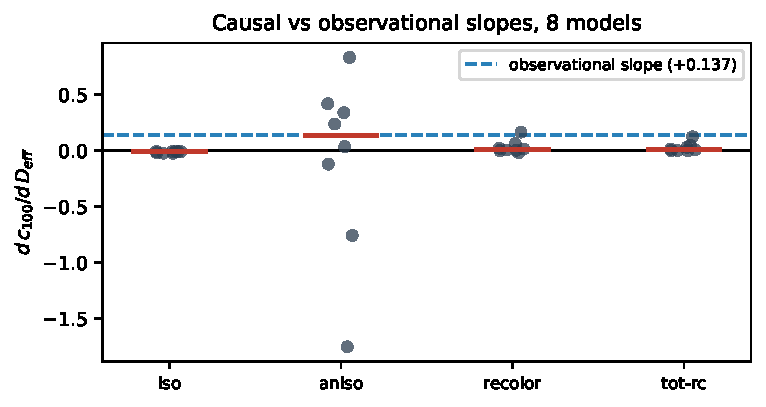
\includegraphics[width=0.82\linewidth]{figs/fig2_slopes.pdf}
\caption{Per-model causal slopes $d c_{100}/d\dfx$ by operator family
(Table~\ref{tab:e1slopes} as a scatter). The dashed line is the
observational slope ($+0.137$); every zero-noise family's slopes cluster
near zero far below it, while the \aniso{} slopes are unstable because
\aniso{} pins $\dfx$ (near-zero denominator). The dose--response harm
signal lives in the \aniso{} \emph{endpoints}
(Figure~\ref{fig:dissociation}), not in per-unit slopes.}
\label{fig:slopes}
\end{figure}

\paragraph{The 3$\times$2 grid closes.}
The decisive cell is \aniso, and it is dose--response, not an endpoint
anecdote: harm grows monotonically with dose in \textbf{8/8} models
(median $\Delta c_{100} = -5.4$ at $\alpha{=}0.5$, $-7.1$ at $\alpha{=}1$,
$-10.8$\,pp at $\alpha{=}2$) while $\dfx$ stays within $11\%$ of baseline
at every dose in 6/8 models (a seventh touches $-11.1\%$ at one dose). The
single outlier ($\dfx$ $+44\%$ at
$\alpha{=}2$) sits \emph{on} the same monotone harm curve ($-13.0$\,pp,
between the $-10.8$ median and the worst model) --- its geometry moved
and its transfer did not benefit, so the harm does not care whether
$\dfx$ moves. At $\alpha{=}2$, $\Delta c_{100}$ median $= -10.8$\,pp
(\textbf{8/8} negative; mean $-11.0$\,pp, paired $d_z = -7.3$), with ID
probe accuracy dropping in lockstep
(median $-12.7$\,pp, 8/8). Meanwhile \rot, which preserves the spectrum
exactly, moves nothing (max $|\Delta c_{100}| = 1.7$\,pp; max
$|\Delta\dfx| = 0.21$). So the harm tracks the \emph{noise}, not the
dimensionality: at essentially pinned $\dfx$, stochasticity alone destroys
both ID and OOD probes; at zero noise, whitening multiplies $\dfx$ by
$1$--$8\times$ and \emph{never} moves transfer below baseline (per-model
$-0.03$ to $+5.6$\,pp). The largest \isot dose (2$\times$ power)
raises $\dfx$ by a median $+5.8$ while \emph{lowering} transfer by
6.5\,pp (8/8) --- the wrong-signed giant movement that definitively kills a
monotone causal reading. Figure~\ref{fig:slopes} shows the per-family
slope distributions against the observational slope;
Figure~\ref{fig:dissociation} summarizes the three
endpoint cells.

\begin{figure}[t]
\centering
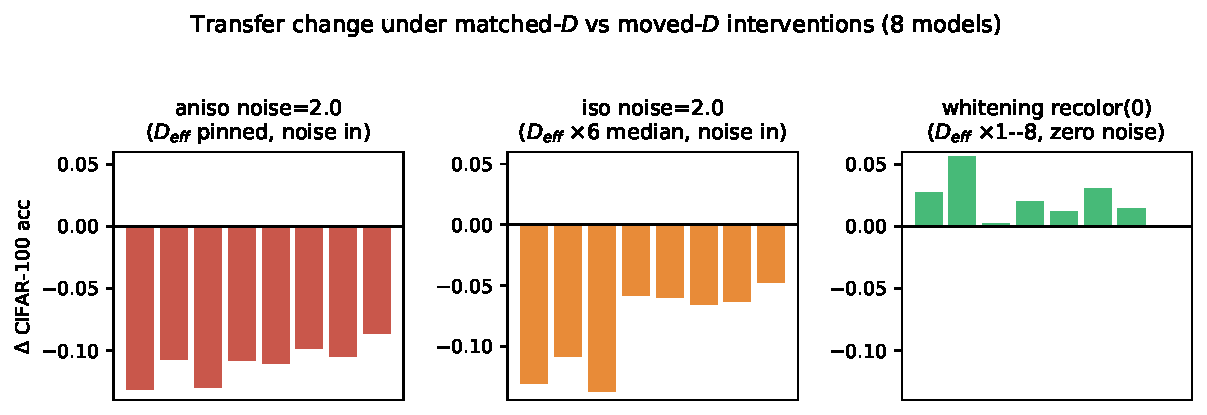
\includegraphics[width=\linewidth]{figs/fig1_dissociation.pdf}
\caption{Per-model transfer change under the three decisive endpoint
interventions (8 ResNet-18 models). \emph{Left}: spectral-shape-matched noise
pins $\dfx$ yet destroys transfer and ID probes alike. \emph{Center}:
isotropic noise \emph{raises} $\dfx$ six-fold and lowers transfer --- the
wrong-signed movement. \emph{Right}: zero-noise whitening multiplies $\dfx$ by $1$--$8\times$ and
leaves transfer non-negative (slightly positive in 7/8 models).
No monotone causal map from $\dfx$ to transfer survives these three cells.}
\label{fig:dissociation}
\end{figure}

\paragraph{Quantifying the causal path.}
The canonical share is defined on the \recolor{} family alone (matching the
permutation floor below and the cross-architecture definition of
Table~\ref{tab:e2arch}): the geometric causal slope is $+0.0105$ pp per unit
$\dfx$, i.e.\ $7.7\%$ of the observational $+0.137$ (bootstrap 95\% CI
$[0.9\%, 46\%]$, wide because $n=8$; pooling the total-spectrum variant
per model gives $10\%$, CI $[2\%, 34\%]$), and the
within-model permutation noise floor for this share is $[-7\%, +7\%]$ ---
the point estimate sits at the floor's upper edge, and even the CI upper
bound leaves half of the observational association without a causal
geometric account.
Across architectures the share is $3.3\%$, $1.9\%$, $-8.3\%$, $+6.0\%$
(ResNet-34/50, ShuffleNet-V2, RegNetY-400MF); the sign flips across
families while the observational anchor stays at $r \ge 0.87$
(Section~\ref{sec:e2}), so the sign instability is itself evidence of
absence. The observational
correlation therefore cannot be recombined from geometry alone: most of
it is recipe-level confounding, and a direct noise channel contributes
with the \emph{opposite} sign to the naive reading. A pilot round of
feature-space interventions (flatten-style dimensionality expansion on
the same 8 models) had already exhibited this sign flip---large $\dfx$
increases paired with monotone transfer losses---which motivated the
preregistered battery reported here; the pilot protocol and its
sign-flip analysis are archived in the released probe reports.

\section{E3: timing separation}
\label{sec:e3}

\subsection{Design}
Paired arms per model. \emph{Formation arm}: recolor $60\%$ of the ID training
features to $\gamma{=}0$ (whitened), freeze the trunk, refit a fresh linear
head \emph{on the whitened features} with the shared probe protocol; evaluate
the resulting representation by CIFAR-100 probe in the whitened space.
\emph{Control arm}: identical subset, identical protocol, no whitening;
evaluate in the original space; additionally evaluate the control features
under the fixed whitened-space probe for the transfer comparison
($c_{100}^{\text{ctrl}}$). \emph{Inference arm} (measurement): apply
\recolor$(0)$ to features and score the \emph{original} trained head ---
the ``geometry as a knob'' usage.

\subsection{Results}
Formation-phase whitening \emph{improves} the transfer measurement:
$\Delta c_{100}$ median $= +1.7$\,pp (7/8 positive, Holm-adjusted Wilcoxon
$p = 0.016$;
mean $+2.0$\,pp, paired $d_z = 1.1$). The inference-arm application
consistently \emph{hurts} the original head: applying \recolor$(0)$ at
inference to the unchanged head is negative in 7/8 models (Holm-adjusted
$p = 0.016$, $d_z = -1.1$), with a small median magnitude of $-0.13$\,pp
--- directionally robust, far below the preregistered collapse threshold
(Appendix~\ref{app:prereg}) --- and the whitened-formation head scored on
original features loses a median $0.35$\,pp vs.\ the control head (8/8
negative, $p = 0.008$).

\paragraph{Mechanism adjudication (dose--response).}
The formation benefit demands a mechanism verdict before any
``geometry helps when acted on early'' reading is allowed
(falsification criteria preregistered in Appendix~\ref{app:prereg},
written before the dose data). We repeat the pipeline at three whitening
doses $\gamma \in \{0.75, 0, -0.5\}$ with three disjoint arms per dose:
(a) \emph{probe-space-only} --- the CIFAR-100 probe is trained and
evaluated in the dose-transformed space with no formation-phase
manipulation whatsoever; (b) \emph{formation readout} --- the 10-class
head is trained on whitened ID features but scored on \emph{original}
test features; (c) \emph{rotate control} --- the probe-space arm with the
spectrum-preserving rotation instead of whitening. The three models are
stratified representatives of the E3 formation gain (low $+0.2$ / mid
$+3.1$ / high $+5.6$\,pp), selected after the E3 endpoint was seen but
before any dose datum existed (Appendix~\ref{app:prereg}, amendment 1).
The verdict is
unambiguous: arm (a) alone reproduces the entire dose--response profile
(cross-model median gain $+1.9$, $+3.1$, $+3.0$\,pp at
$\gamma \in \{0.75, 0, -0.5\}$, monotone to the $\gamma{=}0$ peak; per
model: $+3.8$/$+5.6$/$+3.7$, $+0.3$/$+0.2$/$-1.0$,
$+1.9$/$+3.1$/$+3.0$\,pp --- the weakest-gain model is flat-to-negative
across doses), arm (b) shows no benefit at any dose in
any model (cross-dose range $+0.1$ to $-11.5$\,pp; the only positive cell,
$+0.11$\,pp, is the smallest dose on the highest-anchor model --- and the
harms \emph{grow} with whitening strength, the opposite of the arm-(a)
dose--response), and arm (c) shows none either
($-0.1$ to $-0.8$\,pp). A norm-matched random-direction perturbation of
the formation set (the placebo control) destroys head training in
$7$/$9$ model--dose cells (final accuracy $0.10$ = chance; the two
surviving cells are the smallest dose at the two lr-$0.125$ models),
confirming the whitening benefit is not generic
perturbation regularization. \emph{The formation benefit is therefore a
probe-conditioning effect, not a representational one}: whitening
flattens the covariance spectrum of the probe's own training space,
which changes the optimization landscape of a 100-class linear head
(direct conditioning measurements in Appendix~\ref{app:e5c}: whitening
reduces the in-rank condition number by up to six orders of magnitude
and lowers the reachable training loss at convergence, though it
initially slows early optimization) --- a measurement
condition, not a representational improvement. The MLP-probe control
(Appendix~\ref{app:e5d}) corroborates this: under a 2-hidden-layer MLP
readout the whitening benefit vanishes ($+1.1$ and $-3.3$\,pp) while the
aniso harm grows ($-15.2$ and $-16.4$\,pp). The preregistered
cross-architecture falsifier (two ShuffleNet-V2 recipes) also upholds the
conclusion --- and sharpens it: in that family the probe-space arm shows
no positive benefit at any dose (at most $+1.0$\,pp), and the
over-whitening dose $\gamma{=}-0.5$ turns clearly negative (down to
$-3.9$\,pp), so
the conditioning effect is an optimization detail of the ResNet-18
feature spectrum, neither representational nor universal.

\paragraph{Revised E3 reading.}
Layered on E1, the phase dependence is real but its mechanism is
measurement-level: whitened spaces are \emph{easier to probe} (a linear
readout trains better there) and \emph{harder to transplant into} an
existing head trained on the original geometry (features stop matching
its weight space). Neither behavior is derivable from the static value
of $\dfx$, and neither constitutes acting on representation geometry
Figure~\ref{fig:phases}. We flag explicitly: the naive reading of the
left panel --- ``whitening during formation improves the model'' --- is
falsified by arm (b).

\begin{figure}[t]
\centering
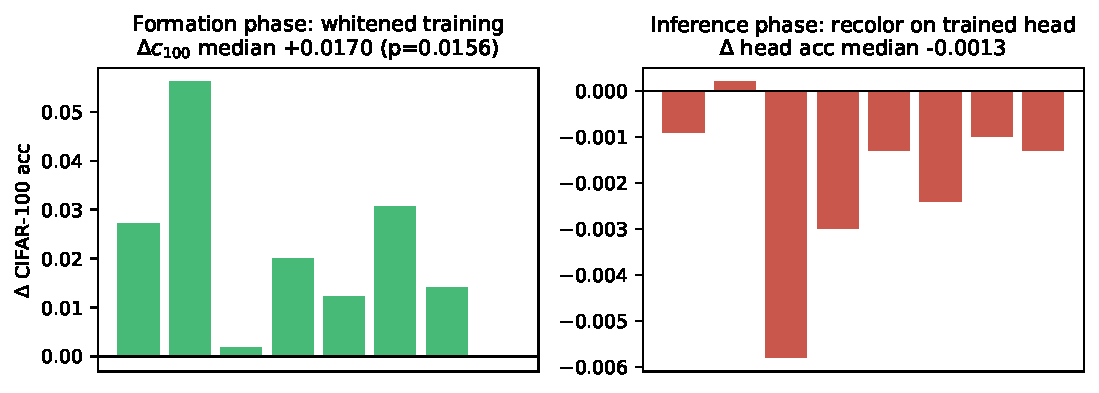
\includegraphics[width=\linewidth]{figs/fig3_phases.pdf}
\caption{Phase separation of the identical whitening operator (8 paired
models). \emph{Left}: whitening the probe space slightly \emph{improves}
the measured CIFAR-100 probe (7/8 positive) --- but the dose--response
adjudication below shows this benefit is fully reproduced without any
formation-phase manipulation: it is a probe-conditioning effect, not a
representational one. \emph{Right}: the same operator applied at
inference to the unchanged trained head consistently \emph{degrades}
accuracy (7/8 negative). The effects live in the measurement, not in the
geometry.}
\label{fig:phases}
\end{figure}

\paragraph{Recipe stratification (post-hoc, exploratory).}
Whitening benefit concentrates in sharper recipes (lr $0.125$:
median $+2.7$\,pp; lr $0.5$: median $+2.0$\,pp) over the sharpest
(lr $1.0$: median $+0.7$\,pp, with one model at $-0.03$\,pp); the single
negative model is the lr-$1.0$/wd-$5\mathrm{e}{-5}$ recipe, whose baseline
$\dfx$ ($0.87$) is the \emph{smallest} in the grid. Two accounts suggested
themselves --- operator saturation at this recipe, and high-$\dfx$ models
having little headroom --- and we have now tested both directly
(Appendix~\ref{app:e5e}), by measuring the probe-space conditioning and the
probe training curve in the original versus dose-whitened space for all
eight paired models. The saturation account survives in a sharpened form:
the negative model's feature covariance is \emph{already} nearly whitened
(in-rank condition number $294$ in the original space, against
$10^{8}$--$10^{9}$ for the sharpest-recipe models), so the operator has
almost nothing to remove --- and indeed whitening neither improves its
conditioning meaningfully ($22\times$, against a median of
$4.6\times10^{3}\times$ across the other seven models), nor lowers its
reachable training loss ($4.134 \to 4.165$ at epoch 40; one of three
models where the loss fails to drop, the other two being slow-converging
lr-$0.5$ probes), and its direct probe benefit is $+0.08$\,pp, the
smallest of the eight. The
headroom account is \emph{refuted}: across the eight models, baseline
$\dfx$ correlates \emph{positively} with the whitening benefit
(Spearman $\rho = +0.857$, $p = 0.007$; the three high-$\dfx$ models
average $+3.5$\,pp against $+0.9$\,pp for the rest), so high-$\dfx$ models
have \emph{more} room for probe-conditioning benefit, not less.
\emph{The stratification itself was not preregistered}; we report it as
exploratory (the paired-gain bootstrap CI is $[+0.2, +3.1]$\,pp). The full
paired table follows.

\begin{table}[t]
\centering
\small
\setlength{\tabcolsep}{4.5pt}
\caption{E3 paired results (8 ResNet-18 models). $c_{100}^{\mathrm{w}}$:
transfer probe in the whitened space after formation-phase whitening;
$c_{100}^{\mathrm{ctrl}}$: same probe, control arm (original space).
$\Delta$ head (inference): \recolor$(0)$ applied to the unchanged trained
head at inference. Auto-generated; do not edit.}
\label{tab:e3paired}
\eThreePairedTable
\end{table}

\section{E2: architecture transfer}
\label{sec:e2}
We repeat the observational anchor and the two decisive separation cells
(\recolor{} slope; \aniso{} at matched power) in four further families, each
with 4 recipes (lr $\in \{0.125, 0.5\}$, wd $\in \{2\mathrm{e}{-4},
5\mathrm{e}{-5}\}$, seed 0): ResNet-34, ResNet-50, ShuffleNet-V2
$\times$1.0, and RegNetY-400MF. MobileNetV3 was originally planned but
replaced by RegNetY-400MF because its classifier head contains a non-linear
bottleneck after average-pooling, so penultimate features are not the input
space of the linear classifier (Appendix~\ref{app:prereg}).

\begin{table}[t]
\centering
\small
\setlength{\tabcolsep}{4.5pt}
\caption{E2 cross-architecture summary (4 recipes per family, 19 conditions
per model). ``share'': inference-time \recolor{} causal slope as a percentage
of the observational slope. ``noise'': $\Delta c_{100}$ median under
\aniso{} at matched power. All numbers auto-generated from locked data.}
\label{tab:e2arch}
\begin{tabular}{@{}lccccc@{}}
\hline
Architecture & obs.\ $r$ & obs.\ slope & \recolor{} share & noise $\Delta c_{100}$ & noise 4/4? \\
\hline
ResNet-18 (E1)  & $+0.97$ & $+0.137$ & $7.7\%$  & $-10.8$\,pp & 8/8 \\
ResNet-34       & $+0.98$ & $+0.133$ & $3.3\%$  & $-9.6$\,pp  & 4/4 \\
ResNet-50       & $+0.98$ & $+0.087$ & $1.9\%$  & $-11.9$\,pp & 4/4 \\
ShuffleNet-V2   & $+0.89$ & $+0.070$ & $-8.3\%$ & $-13.1$\,pp & 4/4 \\
RegNetY-400M    & $+0.87$ & $+0.114$ & $+6.0\%$ & $-16.0$\,pp & 4/4 \\
\hline
\end{tabular}
\end{table}

Three regularities hold in every family (Table~\ref{tab:e2arch},
Figure~\ref{fig:arch}).
\emph{(i) The anchor survives}: $r(\dfx, c_{100})$ is $+0.98$ in both deeper
ResNets and $+0.87$ to $+0.89$ in the compact families --- modestly weaker,
consistent with narrower recipe grids, but far from the null.
\emph{(ii) The noise channel dominates and ignores $\dfx$}: \aniso{} at
matched power drops transfer $9.6$--$16.0$\,pp (family medians; every
individual model is negative in 16/16, with per-model drops of $8.3$ to
$19.8$\,pp). The $\dfx$ shift at the aniso endpoint is small for most
models ($\le 12\%$ in 10/16; up to $52\%$ in three compact-family models
whose harm is at or above their family median), so the harm does not
track the geometric shift; the drop is \emph{largest} in the
compact families ($-13.1$ and $-16.0$\,pp) whose observational anchors are
weakest --- noise harm and anchor strength dissociate.
\emph{(iii) The geometric causal share stays at the noise floor}:
\recolor{} slopes
span $-8.3\%$ to $+6.0\%$ of the observational slope. Permutation tests
(within each model, permuting $c_{100}$ across the dose ladder destroys any
dose--response structure) place each family's noise floor at
$[-6.9, 6.8]$ (r18), $[-6.9, 5.0]$ (r34), $[-2.5, 43.0]$ (r50),
$[-20.2, 21.7]$ (sfn), and $[-2.8, 4.6]$\% (regnet). Three of the five
shares (ResNet-34, ResNet-50, ShuffleNet) lie inside their floors, so the
cross-family sign wobble (ShuffleNet's is negative) is null structure, not
a small real channel: a channel carrying a causal signal of the size the
observational slope suggests could not flip sign under a family swap while
the observational correlation stays at $r \ge 0.87$. Two shares sit
marginally \emph{above} their floors' upper bounds (ResNet-18 $+7.7\%$ vs.\
$+6.8\%$; RegNetY $+6.0\%$ vs.\ $+4.6\%$), and the ResNet-50 floor is wide
($n{=}4$ slope instability). For these families the null reading does not
rest on the floor alone but on the sign-consistent noise harm (8/8 and
4/4 negative) and the near-zero absolute \recolor{} slopes (r18 $+0.0105$,
r50 $+0.0017$, regnet $+0.0068$ pp per unit $\dfx$, vs.\ observational
$+0.137$/$+0.087$/$+0.114$). The dissociation is
not a ResNet-18 artifact; if anything, the ResNet-18 grid is the
\emph{most} generous setting for the geometric path.

\begin{figure}[t]
\centering
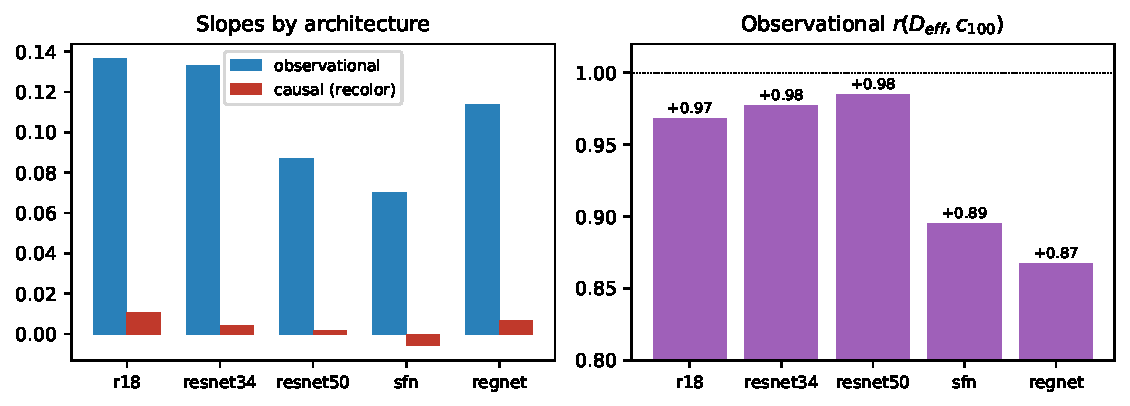
\includegraphics[width=\linewidth]{figs/fig4_arch.pdf}
\caption{Cross-architecture summary (5 families, 24 recipes total).
\emph{Left}: observational vs.\ inference-time causal slopes per
architecture --- the causal bar is a small fraction of the observational bar
everywhere. \emph{Right}: the observational correlation replicates in every
architecture family ($r \ge 0.87$).}
\label{fig:arch}
\end{figure}

\section{E6: marker generality}
\label{sec:e6}
The audit targets one marker. A natural defense of geometry-intervention
methods is that $\dfx$ is the wrong geometry --- participation ratio (PR) or
effective rank might be the manipulable one. We therefore recompute two
further covariance-spectrum markers on the same ID-test subsample for all
152 E1 cells (8 models $\times$ 19 conditions) and ask whether the
dissociation anatomy is $\dfx$-specific.

It is not. Both markers anchor observationally
($r(\mathrm{PR}, c_{100}) = +0.77$, $r(\mathrm{erank}, c_{100}) = +0.86$;
both track $\dfx$ at $r \ge 0.81$). Under \aniso{} at matched power ---
the cell where transfer collapses $10.8$\,pp --- PR \emph{rises} by a
median $+32\%$ and effective rank by $+29\%$: the noise pushes these
geometric markers toward the observationally ``better'' regime while the
model gets monotonically worse, the same wrong-signed movement the
\isot{} cell exposes for $\dfx$, now with the harm cell itself.
Under \recolor$(0)$ both markers move as designed (PR $+92\%$ median,
erank $+144\%$) with the same $\le 2$\,pp transfer neutrality, and \rot{}
pins both exactly (relative change $+0.000$), re-validating the pipeline.
The confounded-label reading is thus not an artifact of one marker's
definition: every spectrum-based geometry descriptor we tested is a
recipe fingerprint, none is a knob.

\section{Discussion: geometry as a label}
\label{sec:discussion}

\paragraph{The slope-decomposition arithmetic.}
Write the observational slope as a sum of channels:
$\beta_{\text{obs}} = \beta_{\text{geo}} + \beta_{\text{recipe}} +
\beta_{\text{noise}}$, where $\beta_{\text{geo}}$ is the direct causal path
from geometry to transfer, $\beta_{\text{recipe}}$ the recipe-level
confounding (the recipe sets both), and $\beta_{\text{noise}}$ any channel
correlated with geometry change but acting through non-geometric means.
Our battery bounds the geometry-only term at a small fraction of the
observational slope
(point estimate $+0.0105$, $7.7\%$ of $\beta_{\text{obs}}$; permutation floor
$[-0.009, +0.009]$, with the point estimate at the floor's upper edge)
and shows that the largest separable non-geometric channel
(noise at matched power) moves transfer \emph{against} the direction its
$\dfx$ change would suggest: $\beta_{\text{noise}} < 0$ while
$\Delta\dfx > 0$ (a $+5.8$ median rise in $\dfx$ accompanies a
$-6.5$\,pp median transfer drop). What remains of the observational
association is recipe confounding. ``Intervene on the geometry'' methods
inherit exactly this arithmetic: no detectable transmission, with a
sign-reversing confounder adjacent to the knob.

\paragraph{What the battery does license.}
Three constructive conclusions survive.
\emph{(i) Noise control.} The only large causal effect we can move transfer
with is noise, and it moves transfer the right way when removed: adding
matched-power noise costs $6$--$11$\,pp at pinned or raised $\dfx$, while
zero-noise operators of comparable geometric magnitude are transfer-neutral.
Spectral-shape-matched noise is the sharpest tool: it is invisible to
$\dfx$ yet costs $11$\,pp---any noise-robustness story that monitors only
geometry will miss it.
\emph{(ii) Formation-time spectral regularization.} Whitening during
formation is mildly transfer-positive ($+1.7$\,pp), concentrated in sharper
recipes. This is a representation-shaping regularizer whose value happens
to co-occur with larger $\dfx$; studying it as a geometry intervention
mistakes the fingerprint for the hand.
\emph{(iii) Observational screening.} The correlation itself replicates
across architectures ($r \ge 0.87$), so $\dfx$ retains value as a cheap
\emph{monitoring} signal for recipe drift---it is the interventional reading
that fails, not the measurement.

\paragraph{A checklist before reading a marker causally.}
The battery reduces to four questions any future ``geometry intervention''
result should answer: (1) \emph{Manipulation check}: does the intervention
realize the intended descriptor change ($r \ge 0.99$ here)? (2)
\emph{Operator separation}: do two operators that move the descriptor
equally but differ in an orthogonal dimension (noise, timing, spectrum)
move the outcome equally? (3) \emph{Negative control}: does a
descriptor-preserving operator (here \rot) leave the outcome unchanged?
(4) \emph{Phase separation}: does the effect survive moving the operator
from formation to inference? A marker whose interventional story survives
all four has earned a causal reading; $\dfx$ passes none.

\paragraph{Relation to the companion papers.}
Paper~1 fixed when the observational link holds (ID-matched,
architecture-adjusted, shift-typed). Paper~2 fixed what the marker measures
(stability map, movement decomposition). Paper~3 (this work) fixes what it
does not do: transmit causal intervention. Together they draw the full
circle from measurement to mechanism.

\section{Limitations}
\label{sec:limitations}
Our conclusions are scoped to: (i) \emph{Scale and dataset}---CIFAR-10
training with CIFAR-100 transfer probes; whether ImageNet-scale recipes
exhibit the same recipe-confounding structure is untested, though the
mechanism (recipes jointly determine geometry and robustness) has no
obvious scale dependence. (ii) \emph{Model count}---8 ResNet-18 recipes
chosen to span the widest $\dfx$ range the recipe grid allows ($2.4\times$),
plus 4 recipes in each of four further
architectures (ResNet-34/50, ShuffleNet-V2, RegNetY-400MF); the observational
anchor and both
separation results replicate in every completed family, but the grid is
not exhaustively factorial. (iii) \emph{Transfer readout}---the anchor and
E1/E2 use linear probes on frozen features (the protocol that makes the
observational anchor clean). The E5d control shows the headline
\emph{harm} results are not linear-probe artifacts --- the aniso damage
\emph{grows} under an MLP readout ($-15$ to $-16$\,pp) --- but the
whitening \emph{benefit} is probe-dependent (it vanishes under MLP), and
full fine-tuning could behave differently still. (iv) \emph{One layer,
one marker family}---all features are penultimate-layer, and although
\S\ref{sec:e6} extends the audit to participation ratio and effective
rank, all three are functions of the same covariance spectrum; discrete or
non-spectral descriptors (e.g.\ uniformity, alignment) are untested.
(v) \emph{Feature-space E3}---formation-phase
whitening acts on penultimate features with a refitted head, not on
weight-space training dynamics; a full-training-run whitening schedule is
the natural extension, and our arm-(b) null makes the burden of proof
explicit for any claim it would help representationally.

\section{Conclusion}
\label{sec:conclusion}
Across three preregistered causal tests, the effective dimension $\dfx$
behaves consistently with a readable fingerprint of the training recipe
rather than a
manipulable cause of OOD generalization: spectral-shape-matched noise
collapses transfer monotonically (by up to $11$\,pp at pinned $\dfx$); moving
$\dfx$ by up to $8\times$ with
zero-noise whitening never moves transfer below baseline ($-0.03$ to
$+5.6$\,pp); the whitening
benefit in formation phase decomposes into probe conditioning, while the
same operator at inference harms; the
entire dissociation replicates across four further architecture families
(24 recipes in total); and two further spectrum markers show the same
anatomy. The observational
correlation---large, stable, and real---transmits to interventions at only a
small fraction of its observational size, at the upper edge of the
permutation noise floor. Methods that reshape
representation geometry to
buy robustness should re-derive their mechanisms in these terms: what
survives the battery is noise control, not geometry targeting. The broader
lesson generalizes
beyond $\dfx$: a strong correlation between a representation descriptor and
a performance outcome is evidence about \emph{what the recipe did}, and
only a battery like this one---operator, phase, and negative controls
together---can say whether the descriptor is also something the recipe can
usefully be asked to change.

\section{Reproducibility statement}
\label{sec:repro}
All experiments run on public CIFAR data with fixed seeds; preregistration in
\texttt{paper/adr\_0016.md} (Appendices 4--5) written before unblinding;
the dose--response falsification criteria (App.~8 + amendment 1) were
committed before any E5 datum existed; the E5b adjudication verdict in
\S\ref{sec:e3} follows those preregistered branches verbatim.
Scripts: \texttt{code/intervene\_v2\_paper.py} (E1--E3),
\texttt{code/intervene\_e5\_dose.py} (E5 dose--response + MLP control),
\texttt{code/intervene\_e5c\_cond.py} (E5c conditioning measurements),
\texttt{code/intervene\_e5d\_ceiling.py} and
\texttt{code/analyze\_e5d\_ceiling.py} (E5e saturation/headroom test),
\texttt{code/intervene\_e6\_marker.py} (E6 second markers),
\texttt{code/intervene\_effect\_probe.py},
\texttt{code/intervene\_recolor.py}; data
\texttt{runs/\{v2\_e1\_full,v2\_e3,v2\_e2\_r34,v2\_e2\_r50,v2\_e2\_sf,%
v2\_e2\_reg,v2\_e5b,v2\_e5d,v2\_e6\}.json};
analysis \texttt{code/paper3\_analysis.py} +
\texttt{code/paper3\_tables.py} + \texttt{code/paper3\_ci.py}
(bootstrap CIs, permutation noise floors, Holm correction)
regenerate every number, figure, and table in this paper from the raw JSON
(\texttt{runs/\{...,v2\_e5b,v2\_e5d,v2\_e5c,v2\_e6\}.json};
and will be released with the code and data archive).

\subsection*{Ethics statement}
This work uses public image datasets and does not involve human subjects.

\subsection*{Use of AI tools}
Large language models were used as writing and coding assistants. All
scientific content, analyses, and reported numbers were determined and
verified by the authors.

\bibliography{references}
\bibliographystyle{tmlr}

\appendix

\section{Preregistration and deviations}
\label{app:prereg}
The experiment matrix and pass/fail criteria below were written and
committed before any v2 number was analyzed (ADR-0016 App.~4, 2026-11-04
morning; scripts committed alongside). We reproduce the criteria verbatim in
substance.

\paragraph{Preregistered matrix.}
E1: 8 ResNet-18 models $\times$ 19 conditions (base;
\isot $\in\{0.5,1,2\}$; \aniso $\in\{0.5,1,2\}$; \rot; scale $\in\{0.5,2\}$;
\recolor $\in\{1.5,0.75,0.5,0.25,0\}$; total-spectrum \recolor
$\in\{0.5,0\}$; placebo $\in\{1,2\}$). The \aniso (spectral-shape-matched
noise) and \rot (spectrum-preserving rotation) cells were preregistered as
the two new separation cells. E2: resnet34 / resnet50 / shufflenet\_v2\_x1\_0
/ mobilenet\_v3\_small $\times$ lr $\in\{0.5,0.125\}$ $\times$
wd $\in\{2\mathrm{e}{-4},5\mathrm{e}{-5}\}$ $\times$ seed 0, merged with the
E1 ResNet-18s for the cross-architecture anchor. E3: same whitening operator
applied (a) at inference vs.\ (b) during formation on a 60\% training
subset with a refit head.

\paragraph{Preregistered criteria.}
\emph{P1}: noise families show per-model $d c_{100}/d\dfx \le -0.05$ with
median $\le -0.05$ and $\ge 6/8$ same sign; zero-noise \recolor{} families
$|$median slope$| \le 0.02$. \emph{P1b}: \aniso{} at matched power with
$|\Delta\dfx|/\dfx \le 0.2$ yields $\Delta c_{100} < 0$ in $\ge 6/8$ models.
\emph{P2}: cross-architecture base $r(\dfx, c_{100}) > 0$ in $\ge 4/5$
architectures, and inference-time \recolor{} slopes $\le 10\%$ of the
observational slope. \emph{P3}: the formation arm lands within
$\pm 0.01$ of base $c_{100}$ with ID head intact, while the inference arm
degrades by $\ge 0.1$ --- phases separable.

\paragraph{Deviations.}
(1) E2 dropped mobilenet\_v3\_small in favor of regnet\_y\_400mf: the
MobileNetV3 head \citep{howard2019searching} contains a non-linear
bottleneck after average-pooling, so penultimate features are not the input
space of the linear classifier and feature-space operators would not act on
the classifier's input. RegNetY-400MF \citep{radosavovic2020designing} was
chosen as a hook-clean lightweight replacement of the same
efficiency-oriented family. (2) E3 protocol was revised twice
\emph{before any E3 number was analyzed}: a first head-finetuning variant
diverged on both arms (train accuracy 0.15--0.36), and a second variant
omitted \texttt{model.eval()}, letting batch-norm use batch statistics and
contaminate round-1 features. The final protocol (head re-initialization +
per-dimension standardization + lr $10^{-2}$, matching E1's verified probe)
was locked before unblinding; both failed variants are archived in the
experiment logs. (3) The preregistration anticipated three evaluation GPUs;
two additional GPUs became available mid-run and were used only to
re-shard the \emph{same} preregistered condition matrix, not to add
conditions.

\paragraph{Where the preregistered criteria fail as written.}
Full honesty requires reporting not only passes. \emph{P1} fails as
written: the \isot{} slope median is $-0.008$, far above the $-0.05$
threshold (its $\dfx$ movement is huge, so per-unit slopes are tiny), and
the \aniso{} slope is numerically unstable because \aniso{} pins $\dfx$ by
construction (division by a near-zero denominator). The paper's noise
claim therefore rests on the P1b \emph{endpoint}, which passes cleanly
(8/8 negative, Holm $p = 0.012$), not on P1 slopes. \emph{P2}'s share
bound passes in every family. \emph{P3} fails as written on both
sub-criteria: the formation arm lands at $+0.017$, \emph{outside} the
preregistered $\pm 0.01$ window (in the beneficial direction --- this is
the resurrection channel adjudicated below), and the inference harm,
while directionally consistent (7/8 negative, Holm $p = 0.016$), is
$30\times$ smaller than the preregistered $\ge 0.1$ collapse. We
interpret P3's failure as the criterion being mis-calibrated at
pre-registration time, not as phase separation being absent; the
mechanism adjudication below replaces it.

\paragraph{Amendment 1 (dose--response falsification criteria).}
Written and timestamped \emph{before any E5 datum existed}, after the E3
endpoint but before the dose--response data. Three mechanism hypotheses
for the formation benefit: \emph{H-reg} (generic regularization; predicts
dose-flat gains), \emph{H-geom} (representational transmission; predicts
monotone gains that persist when the whitened representation is scored in
the original space), and \emph{H-cond} (probe conditioning; predicts
monotone gains fully reproduced in the probe's own transformed space,
absent on original-space readouts). Adjudication rule: the paper's
``geometry is not a knob'' conclusion is \emph{withdrawn} if and only if
arm (b) --- whitened-formation representation scored on original
features --- shows monotone in-dose benefits $\ge 0.5$\,pp in all models
replicating across architectures. \emph{Outcome}: arm (b) is flat-null in
every model at every dose; arm (a) reproduces the entire benefit ---
H-cond confirmed, H-reg and H-geom rejected. The conclusion stands.

\section{E1 endpoint summary table}
\label{app:e1table}
Rather than a 152-row dump, we release the full per-cell records as
machine-readable JSON (\texttt{runs/v2/e1/intervene\_v2.json}; 8 models
$\times$ 19 conditions) and summarize the decisive endpoints here.
Table~\ref{tab:e1endpoints} reports per-model endpoint deltas for the three
decisive cells of Figure~\ref{fig:dissociation}.

\begin{table}[h]
\centering
\small
\setlength{\tabcolsep}{4pt}
\caption{E1 per-model endpoint deltas (pp): \aniso$(2)$, \isot$(2)$, and
\recolor$(0)$ vs.\ base. Negative values: transfer loss. The \aniso{} column
is negative in 8/8 models despite $|\Delta\dfx|/\dfx \le 44\%$; the
\recolor$(0)$ column is never negative despite $\dfx$ multiplying
$1$--$8\times$. Auto-generated from the locked data.}
\label{tab:e1endpoints}
\eOneEndpointTable
\end{table}

\section{E5d: MLP-probe control}
\label{app:e5d}
To test whether the E1 findings depend on the linear readout, we repeat the
decisive conditions (base, \recolor$(0)$, \aniso$(2)$, \rot) on two
representative models with a 2-hidden-layer (512, 512, ReLU) probe under the
identical optimization protocol. The \emph{harm} results strengthen:
\aniso$(2)$ costs $-15.2$ and $-16.4$\,pp under the MLP (vs.\ $-9.9$ and
$-10.7$\,pp linear) --- the noise damage is not an artifact of linear
readout. \rot{} remains small ($-1.6$, $-3.9$\,pp). The whitening
\emph{benefit} disappears ($+1.1$ and $-3.3$\,pp vs.\ $+3.1$ and $+5.6$\,pp
linear), consistent with the probe-conditioning account of
\S\ref{sec:e3}: whitening eases \emph{linear} probe optimization
specifically. We flag that this control covers two models only; it
establishes direction, not precise magnitudes.

\section{E5e: direct test of the saturation and headroom conjectures}
\label{app:e5e}
\emph{Exploratory} (not preregistered; added to convert the two
conjectures of the E3 stratification into measurements). We repeat the
E5c protocol --- conditioning statistics of the probe-train covariance and
the 40-epoch shared-protocol probe training curve, in the original versus
the $\gamma{=}0$ dose-whitened space --- on \emph{all eight} E3 paired
models rather than the three E5b models (three of the eight overlap E5c
and reproduce its conditioning numbers and final accuracies under
seed-pinned reruns; the condition numbers agree exactly in 15/18
conditions and to floating-point tolerance in all 18, the residual
differences coming from BLAS-level eigenvalue tail bits).

The two conjectures fare differently.

\emph{Operator saturation (supported, sharpened).} The model that showed
no E3 benefit (lr-$1.0$/wd-$5\mathrm{e}{-5}$, baseline $\dfx=0.87$, the
smallest in the grid) has an original-space in-rank condition number of
$294$ --- three to seven orders of magnitude below the other seven models
($10^{3}$--$10^{9}$). Its covariance is already nearly whitened, so the
operator has almost nothing to remove: whitening improves its conditioning
by only $22\times$ (median across the other seven:
$4.6\times10^{3}\times$), fails to lower its reachable training loss
($4.134 \to 4.165$ at epoch 40; one of three models where the loss does
not drop, the other two being slow-converging lr-$0.5$ probes), and
yields the smallest direct probe benefit of the eight ($+0.08$\,pp).
Saturation at this recipe is therefore not a
property of the operator but of the representation: the recipe trained a
representation whose probe-space spectrum was already flat.

\emph{High-$\dfx$ headroom (refuted).} Across the eight models, baseline
$\dfx$ correlates \emph{positively} with the direct whitening benefit at
$\gamma{=}0$ (Pearson $r = +0.743$, Spearman $\rho = +0.857$,
$p = 0.007$): the three high-$\dfx$ models ($\dfx \ge 11$) average
$+3.5$\,pp of probe benefit against $+0.9$\,pp for the five
lower-$\dfx$ models. Whatever limits the benefit at the lr-$1.0$
recipes, it is not exhaustion of the high-$\dfx$ models' headroom ---
recipe sharpness, not geometry, is what correlates with the benefit's
absence, consistent with the dose--response adjudication of
\S\ref{sec:e3}. Data: \texttt{runs/v2\_e5d\_ceiling/intervene\_e5d\_ceiling.json}.

\section{E5c: direct conditioning measurements}
\label{app:e5c}
\emph{Exploratory} (not preregistered; added after the E5b adjudication to
turn the conditioning inference into a measurement). For the three E5b
models we train the shared-protocol 100-class linear probe in the original
vs.\ the dose-whitened space (identical 60\% training subset, seed-pinned)
and record (i) conditioning statistics of the probe-train covariance and
(ii) the training curve at epochs $\{1,2,4,8,16,24,32,40\}$.

Because ReLU features are numerically rank-deficient, the raw
$\lambda_{\max}/\lambda_{\min}$ condition number is degenerate; we report
the \emph{in-rank} condition number $\lambda_1/\lambda_r$ instead (the
numerical rank at $\lambda > 10^{-10}\lambda_{\max}$ is itself diagnostic:
$494$--$512$ of $512$ in the two sharper-recipe ResNet-18 models, but only
$99$--$122$ of $512$ in the lr-$0.5$ model, rising to $106$--$122$ after
whitening --- whitening raises the usable rank there). At
$\gamma{=}0$ whitening reduces the in-rank condition number by
$10^{2}$--$10^{6}\times$
(e.g.\ $2.8{\times}10^{9} \to 8.4{\times}10^{3}$ in
{\tt l0.125\_w0.0002\_s2}), and partial doses interpolate
($\gamma{=}0.75$: $9.3{\times}10^{7}$). Two honest qualifications:
first, the conditioning improvement does not track the
probe-space benefit monotonically across models (the {\tt l0.5\_w5e-05\_s2}
model shows only a $1.9\times$ reduction yet a $+2.1$\,pp benefit, so the
benefit is not a pure condition-number effect); second, whitening
\emph{slows early optimization} (epoch-1 training loss $4.05 \to 4.50$,
epoch-1 accuracy $8.8\% \to 3.7\%$, consistent with the standardization
in the probe protocol partially undoing the whitening early in training)
while lowering the \emph{reachable} loss at convergence
(epoch-40 training loss $3.43 \to 3.01$ in the same model, and lower
train loss at convergence in 8/9 model--dose pairs; the exception is the
smallest benefit model at the $\gamma{=}-0.5$ dose). The probe-conditioning
account of \S\ref{sec:e3} therefore survives the direct measurement in a
sharpened form: whitening changes where probe optimization can
\emph{end}, not how fast it starts --- a property of the measurement
space, not of the representation. Data: \texttt{runs/v2\_e5c.json}.

\end{document}
